\documentclass[../main/report.tex]{subfiles}
\begin{document}

\section{Input}

The main method of communication between the microcontroller and a host PC is USB.
However, if the usb fail, a serial port(RS-232) has been implemented as a backup solution.
If this also fails, the wires from the serial port is put on headers, which can be used as GPIO pins.

\begin{figure}[H]
		\centering
		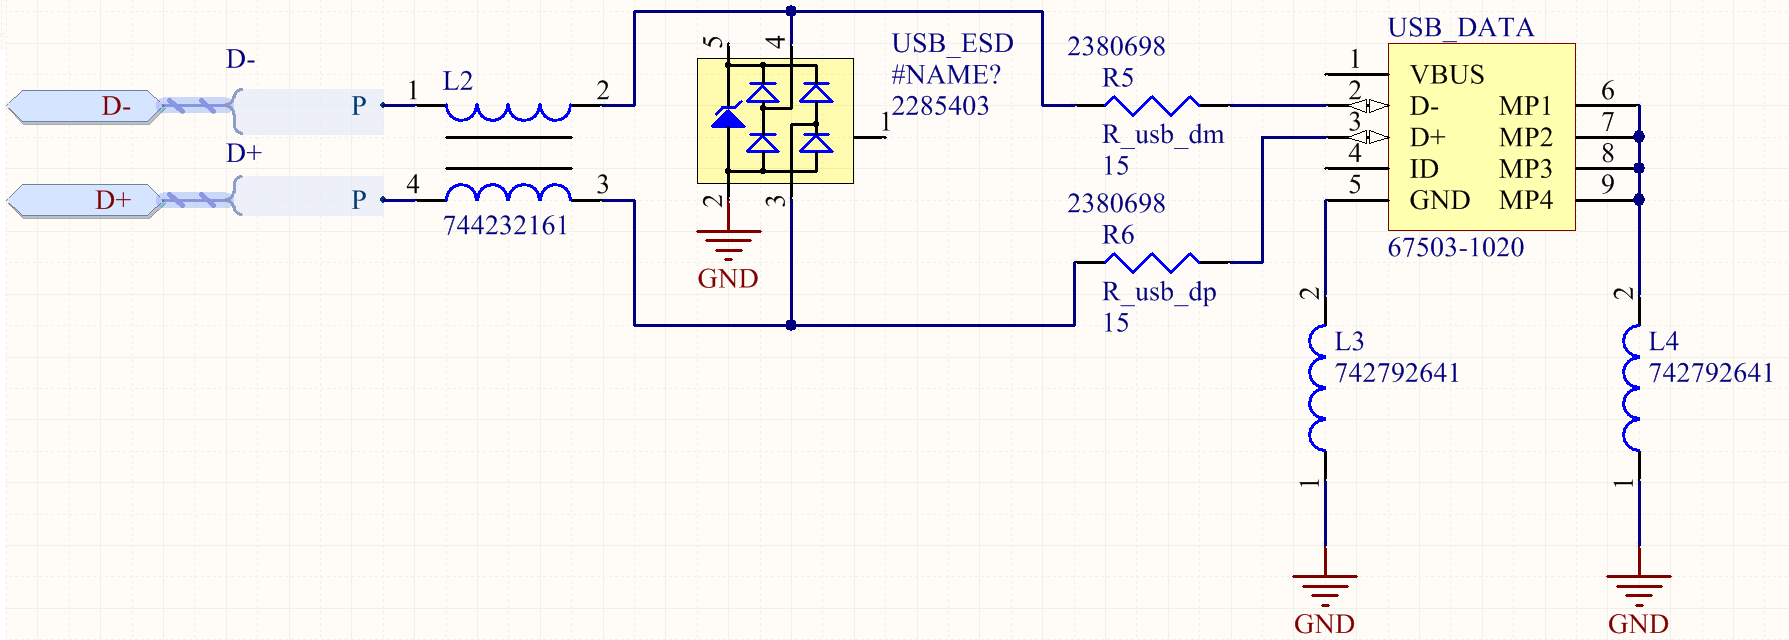
\includegraphics[width=0.75\textwidth]{../pcb/assets/input.png}
		\caption{Data input circuit}
		\label{fig: input circuit}
\end{figure}
\end{document}
